\documentclass{article}
\usepackage{graphicx,float}
\usepackage{amsmath,latexsym,amsfonts,amssymb,amsthm}

\usepackage[utf8]{inputenc}
\usepackage[english]{babel}
\usepackage[letterpaper,top=2cm,bottom=2cm,left=3cm,right=3cm,marginparwidth=1.75cm]{geometry}
\renewcommand{\baselinestretch}{1.667}


\title{Introduction To Quantum Computing PS s7 Lab}
\author{Joris Plaščinskas}
\date{\today}


\begin{document}


    \maketitle
    \section*{Lab 1.1}
        \subsection*{Exercise 1-5}
            Simplify: \\
            \begin{math}
                ((\frac{1}{-i}) + (\frac{1}{-i})^2 + (\frac{1}{-i})^3 + \cdots +  (\frac{1}{-i})^{30})^{-3} = (i + i^{2} + i^{3} + ... + i^{30} )^{-3} = ((i + i^{2} + i^{3} + i^{4}) + i^{5} + ... + i^{30} )^{-3} = (i^{29} + i^{30})^{-3} = (i^{1} + i^{2})^{-3} = (i - 1)^{-3} = \frac{1}{(i - 1)^{3}} = \frac{1}{(-1+i)*(-1+i)*(-1+i)} = \frac{1}{-2i * (-1+i)} = \frac{1}{2 + 2i} = \frac{1 - i}{4}
            \end{math}

            
        \subsection*{Exercise 2-5}
            \begin{math}
                u + \overline{w}^2 + \frac{|z|}{|z+1|^2} = (1 + i) + (\overline{1 - i})^2 + \frac{|1 + 2i|}{| (1 + 2i) + 1 |^2} = (1 + i) + (1 + i)^2 + \frac{\sqrt{1^2 + (2)^2}}{|2 + 2i|^2} = (1 + i) + [1 + 2i + i^2] + \frac{\sqrt{5}}{(\sqrt{(2)^2 + (2)^2})^2} = (1 + i) + [1 + 2i - 1] + \frac{\sqrt{5}}{(\sqrt{8})^2} = (1 + i) + [2i] + \frac{\sqrt{5}}{8} = 1 + i + 2i + \frac{\sqrt{5}}{8} = \left(1 + \frac{\sqrt{5}}{8}\right) + 3i
            \end{math}

            
        \subsection*{Exercise 3-5}
            \paragraph{Given the complex number:}\leavevmode\\
            \begin{math}
                z = -30 \sqrt{2} - 10\sqrt{6} i
            \end{math}
            \paragraph{Find the modulus \( r \):}\leavevmode\\
            \begin{math}
                r=\sqrt{\left(Re(z)\right)^2+\left(Im(z)\right)^2}=\sqrt{\left(-30\sqrt{2}\right)^2+\left(-10\sqrt{6}\right)^2}=\sqrt{\left(900\times2\right)+\left(100\times6\right)}=\sqrt{1800+600}=\sqrt{2400}=\sqrt{16\times150}=4\sqrt{150}=4\sqrt{25\times6}=4\times5\sqrt{6}=20\sqrt{6}
            \end{math}
            \paragraph{Find the argument $\theta$:}\leavevmode\\
            \begin{math}
                \theta=\arctan\left(\frac{Im(z)}{Re(z)}\right)-\pi=\arctan\left(\frac{-10\sqrt{6}}{-30\sqrt{2}}\right)-\pi=\frac{\pi}{6}-\pi=-\frac{5\pi}{6}
            \end{math}
            \paragraph{So the exponent form is:}\leavevmode\\
            \begin{math}
                z=re^{\theta i}=20\sqrt{6}e^{(-\frac{5\pi}{6})i}
            \end{math}

            
        \subsection*{Exercise 4-15}
            Find x: 
            \begin{math}
                3x^2+3x+30=0\\
                D=b^2-4ac=3^2-4*3*30=-351\\
                \sqrt{-351}=3\sqrt{39}*i\\
                x_{1,2}=\frac{-3\pm3\sqrt{39}*i}{2*3}=-0,5\pm0,5\sqrt{39}*i
            \end{math}

            
        \subsection*{Exercise 5-15}
            Given: 
            \begin{math}
                n=9,z=-64i,\sqrt[9]{-64i}=?\\
                64e^{-\frac{\pi}{2}i}\\
                r^9=64\\
                r=\sqrt[9]{64}\\
                n\theta=\theta_{0}+2\pi k\\
                \theta=\frac{-\frac{\pi}{2}+2\pi k}{9}; k=0,1,2,...,8\\\
                z_{0}=64^{2/3}e^{-\frac{\pi}{18}i}\\
                ...\\
                z_{8}=...
            \end{math}

            
        \subsection*{Exercise 6-5}
            \begin{math}
                2 \leq |z+1-i| \leq 10, \Im(z) < 1\\
                2 \leq |x+y+1-i| \leq 10\\
                2 \leq \sqrt{(x+1)^2+(y-1)^2} \leq 10\\
                4 \leq (x+1)^2+(y-1)^2 \leq 100\\
            \end{math}
            \begin{figure}[H]
                \centering
                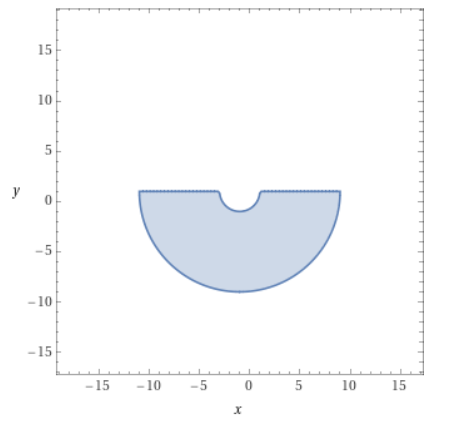
\includegraphics[width=0.6\textwidth]{graph.png}
                \caption{Solutions graph}
                \label{fig:solutions-graph}
            \end{figure}
    \newpage
    
    
    \section*{Lab 1.2}
        This part of the lab is very computations heavy. Therefore some of the calculations will be performed using python (numpy, scipy).
        \subsection*{Exercise 1-15}
            Are the given vectors: 
            $
                \vec{v_1} = 
                \begin{bmatrix} 1 - i \\ -4 - 4i \\ -4 - 3i \\ 2 - 5i \end{bmatrix}
            $, 
            $
                \vec{v_2} = \begin{bmatrix} -3 - 3i \\ -4 + i \\ -2 + 2i \\ -3 - 4i \end{bmatrix}
            $, 
            $
                \vec{v_3} = \begin{bmatrix} -3 - i \\ -2 + 3i \\ -4 - 3i \\ -5 - 4i \end{bmatrix}
            $ 
            linearly independent? \\
            If the vectors are linearly independent, then the equation below is only true, when $\alpha_1$, $\alpha_2$, $\alpha_3$ are all equal to 0:
            \[
                \alpha_1 
                \begin{bmatrix}
                    1 - i \\
                    -4 - 4i \\
                    -4 - 3i \\
                    2 - 5i
                \end{bmatrix}
                +
                \alpha_2
                \begin{bmatrix}
                    -3 - 3i \\
                    -4 + i \\
                    -2 + 2i \\
                    -3 - 4i
                \end{bmatrix}
                +
                \alpha_3
                \begin{bmatrix}
                    -3 - i \\
                    -2 + 3i \\
                    -4 - 3i \\
                    -5 - 4i
                \end{bmatrix}
                =
                \begin{bmatrix}
                    0 \\
                    0 \\
                    0 \\
                    0
                \end{bmatrix}
            \]
            \[
                \begin{bmatrix}
                    \alpha_1 * (1 - i) + \alpha_2 * (-3 - 3i) + \alpha_3 * (-3 - i)\\
                    \alpha_1 * (-4 - 4i) + \alpha_2 * (-4 + i) + \alpha_3 * (-2 + 3i)\\
                    \alpha_1 * (-4 - 3i) + \alpha_2 * (-2 + 2i) + \alpha_3 * (-4 - 3i)\\
                    \alpha_1 * (2 - 5i) + \alpha_2 * (-3 - 4i) + \alpha_3 * (-5 - 4i)
                \end{bmatrix}
                =
                \begin{bmatrix}
                    0 \\
                    0 \\
                    0 \\
                    0
                \end{bmatrix}
            \]
            \[
                \begin{bmatrix}
                    1 - i & -3 - 3i & -3 - i\\
                    -4 - 4i & -4 + i & -2 + 3i\\
                    -4 - 3i & -2 + 2i & -4 - 3i\\
                    2 - 5i & -3 - 4i & -5 - 4i
                \end{bmatrix}
                \cdot 
                \begin{bmatrix}
                    \alpha_1\\
                    \alpha_2\\
                    \alpha_3
                \end{bmatrix}
                = 
                \begin{bmatrix}
                    0\\
                    0\\
                    0\\
                    0
                \end{bmatrix}
            \]
            We can rewrite this and solve using Gaussian elimination method
            \[
                \begin{bmatrix}
                    1 - i & -3 - 3i & -3 - i & | 0\\
                    -4 - 4i & -4 + i & -2 + 3i & | 0\\
                    -4 - 3i & -2 + 2i & -4 - 3i & | 0\\
                    2 - 5i & -3 - 4i & -5 - 4i & | 0
                \end{bmatrix}
            \]
            1st Gaussian elimination step
            \begin{align*}
                m_2 &= \frac{-4-4i}{1-i} = \frac{(-4-4i)*(1+i)}{1^2+1^2} = \frac{-4-4i-4i+4}{2} = -4i \\
                m_3 &= \frac{-4-3i}{1-i} = \frac{(-4-3i)*(1+i)}{2} = \frac{-4-4i-3i+3}{2} = -\frac{1+7i}{2} \\
                m_4 &= \frac{2-5i}{1-i} = \frac{(2-5i)*(1+i)}{2} = \frac{2+2i-5i+5}{2} = \frac{7-3i}{2}
            \end{align*}
            \begin{itemize}
                \item Row 1 scaling by $m_2$: $(3-3i) * -4i = -12i-12; (-3 - i) * -4i = 12i-4$
                \item Row 2 subtraction: $-4+i - (-12i-12) = 8+13i; -2+3i - (12i-4) = 2-9i$
                \item Row 1 scaling by $m_3$: $(3-3i)*(-0,5-3,5i) = -1,5-10,5i+1,5i-10,5 = -12-9i; (-3-i)*(-0,5-3,5i) = -2+11i$
                \item Row 3 subtraction: $-2+2i - (-12-9i) = 10+11i ; -4-3i - (-2+11i) = -2-14i$
                \item Row 1 scaling by $m_4$: $(-3-3i) * \frac{7-3i}{2} = -15-6i; (-3-i) * \frac{7-3i}{2} = -12+i$
                \item Row 4 subtraction: $-3-4i - (-15-6i) = 12+2i; -5-4i - (-12+i) = 7-5i$
            \end{itemize}
            Resulting matrix:
            \[
                \begin{bmatrix}
                    1 + i & 3 - 3i & -3 - i & | 0\\
                    0 & 8+13i & 2-9i & | 0\\
                    0 & 10+11i & -2-14i & | 0\\
                    0 & 12+2i & 7-5i & | 0
                \end{bmatrix}
            \]
            2nd Gaussian elimination step
            \begin{align*}
                m_3 &= \frac{10+11i}{8+13i} = \frac{223}{233} - \frac{42}{233}i\\
                m_4 &= \frac{12+2i}{8+13i} = \frac{122}{233} - \frac{140}{233}i
            \end{align*}
            \begin{itemize}
                \item Row 2 scaling by $m_3$: \\ $(8+13i)*(\frac{223}{233} - \frac{42}{233}i) = 10 + 11i; \\ (2-9i)*(\frac{223}{233} - \frac{42}{233}i) = \frac{68}{233} - \frac{2091}{233}i$
                \item Row 3 subtraction: \\$10+11i - (10 + 11i) = 0; \\
                -2-14i - (\frac{68}{233} - \frac{2091}{233}i) = -\frac{534}{233} - \frac{1171}{233}i$
            \end{itemize}
            \[
                \begin{bmatrix}
                    1 + i & 3 - 3i & -3 - i & | 0\\
                    0 & 8+13i & 2-9i & | 0\\
                    0 & 0 & -\frac{534}{233} - \frac{1171}{233}i & | 0\\
                    0 & 12+2i & 7-5i & | 0
                \end{bmatrix}
            \]
            \[
                \begin{bmatrix}
                    1 + i & 3 - 3i & -3 - i & | 0\\
                    0 & 8+13i & 2-9i & | 0\\
                    0 & 0 & 1 & | 0\\
                    0 & 12+2i & 7-5i & | 0
                \end{bmatrix}
            \]
            \[
                \begin{bmatrix}
                    1 + i & 3 - 3i & -3 - i & | 0\\
                    0 & 8+13i & 0 & | 0\\
                    0 & 0 & 1 & | 0\\
                    0 & 12+2i & 7-5i & | 0
                \end{bmatrix}
            \]
            \[
                \begin{bmatrix}
                    1 + i & 0 & 0 & | 0\\
                    0 & 8+13i & 0 & | 0\\
                    0 & 0 & 1 & | 0\\
                    0 & 12+2i & 7-5i & | 0
                \end{bmatrix}
            \]
            \[
                \begin{bmatrix}
                    1 & 0 & 0 & | 0\\
                    0 & 1 & 0 & | 0\\
                    0 & 0 & 1 & | 0\\
                    0 & 0 & 0 & | 0
                \end{bmatrix}
            \]
            $\alpha_1 = 0,\alpha_2 = 0,\alpha_3 = 0$, this means that the vectors are linearly independent.

            
        \subsection*{Exercise 2-15}
            Find: $A^2 + 3B^{\dagger}C^{-2} + (A^{-1})^{\dagger}$.
            \[
                \text{When: }
                A=\left[\begin{matrix}-4 + 8 i & 2 + 5 i\\-3 + 7 i & 2 + 2 i\end{matrix}\right], B=\left[\begin{matrix}-3 - 6 i & -7 - i\\7 - 5 i & -2 + i\end{matrix}\right], C=\left[\begin{matrix}2 - 5 i & -4 - 5 i\\-5 + i & -9 - 4 i\end{matrix}\right]
            \]
            We will first find $A^{-1}$
            \[
                \begin{bmatrix}
                    -4 + 8 i & 2 + 5 i & | & 1 & 0\\
                    -3 + 7 i & 2 + 2 i & | & 0 & 1\\
                \end{bmatrix}
            \]

            \[
                \begin{bmatrix}
                    1 & \frac{(2 + 5 i)}{(-4 + 8 i)} & | & \frac{1}{(-4 + 8 i)} & 0\\
                    0 & (2 + 2 i) - (\frac{(2 + 5 i)}{(-4 + 8 i)} * (-3 + 7 i)) & | & \frac{-3 + 7 i}{(4 - 8 i)} & 1\\
                \end{bmatrix}
            \]
            \[
                \begin{bmatrix}
                    1 & \frac{(2 + 5 i)}{(-4 + 8 i)} & | & \frac{1}{(-4 + 8 i)} & 0\\
                    0 & \frac{1}{20} - \frac{43}{20}i & | & \frac{-3 + 7 i}{(4 - 8 i)} & 1\\
                \end{bmatrix}
            \]
            \[
                \begin{bmatrix}
                    1 & \frac{(2 + 5 i)}{(-4 + 8 i)} & | & \frac{1}{(-4 + 8 i)} & 0\\
                    0 & 1 & | & \frac{3-7i}{17+9i} & \frac{1}{\frac{1}{20} - \frac{43}{20}i}\\
                \end{bmatrix}
            \]
            \[
                \begin{bmatrix}
                    1 & 0 & | & \frac{-2+14i}{15+95i} & -((\frac{1}{\frac{1}{20} - \frac{43}{20}i})*(\frac{(2 + 5 i)}{(-4 + 8 i)}))\\
                    0 & 1 & | & \frac{3-7i}{17+9i} & \frac{1}{\frac{1}{20} - \frac{43}{20}i}\\
                \end{bmatrix}
            \]
            \[
                \begin{bmatrix}
                    1 & 0 & | & \frac{26+8i}{185} & -\frac{79}{370} - \frac{67}{370}i\\
                    0 & 1 & | & \frac{-6-73i}{185} & \frac{2}{185} + \frac{86}{185}i\\
                \end{bmatrix}
            \]
            \begin{align*}
                A^{-1} &= 
                \begin{bmatrix}
                    \frac{26}{185} + \frac{8}{185}i & -\frac{79}{370} - \frac{67}{370}i\\
                    -\frac{6}{185} - \frac{73}{185}i & \frac{2}{185} + \frac{86}{185}i\\
                \end{bmatrix}
                \\
                (A^{-1})^{\dagger} &= 
                \begin{bmatrix}
                    \frac{26}{185} + \frac{8}{185}i & -\frac{6}{185} + \frac{73}{185}i\\
                    -\frac{79}{370} + \frac{67}{370}i & \frac{2}{185} + \frac{86}{185}i\\
                \end{bmatrix}
                \\
                A^2 &= 
                \begin{bmatrix}
                    -89-65i & -54+10i\\
                    -64-44i & -41+7i\\
                \end{bmatrix}
                \\
                C^{-2} &= C^{-1}C^{-1} = 
                \begin{bmatrix}
                    \frac{503}{4425} + \frac{396}{4425}i & -\frac{172}{4425} - \frac{379}{4225}i\\
                    -\frac{331}{4225} - \frac{17}{4225}i & -\frac{206}{4225} + \frac{283}{4225}i\\
                \end{bmatrix}
                \begin{bmatrix}
                    \frac{503}{4425} + \frac{396}{4425}i & -\frac{172}{4425} - \frac{379}{4225}i\\
                    -\frac{331}{4225} - \frac{17}{4225}i & -\frac{206}{4225} + \frac{283}{4225}i\\
                \end{bmatrix}
                \\
                C^{-2} &= 
                \begin{bmatrix}
                    \frac{146682}{17850625} + \frac{526749}{17850625}i & \frac{206257}{17850625} - \frac{229351i}{17850625}i\\
                    -\frac{86764}{17850625} - \frac{229798}{17850625}i & \frac{12836}{17850625} + \frac{11777}{17850625}i\\
                \end{bmatrix}
                \\
                B^{\dagger} &= 
                \begin{bmatrix}
                    -3 - 6 i & 7 + 5 i \\
                    -7 + i & -2 + i
                \end{bmatrix}
                \\
                3B^{\dagger} &= 
                \begin{bmatrix}
                    -9 - 18i & 21 + 15i \\
                    -21 + 3i & -6 + 3i
                \end{bmatrix}
            \end{align*}
            So, putting $A^2,3B^{\dagger},C^{-2},(A^{-1})^{\dagger}$ into SciPy, we get this matrix:
            \[
                \begin{bmatrix}
                -88.31 - 65.71i & -54.36 + 10.33i \\
                -64.41 - 44.35i & -41.20 + 7.77i \\
                \end{bmatrix}
            \]

            
        \subsection*{Exercise 3-15}
            Rewrite $\vec{v_4}$ using $\vec{v_1}$, $\vec{v_2}$, $\vec{v_3}$.
            \[
                \begin{bmatrix}
                    2-4i & 2-5i & 2-3i \\
                    -1-3i & -2-i & 4-4i \\
                    -4-4i & -1+3i & 1-5i
                \end{bmatrix}
                \cdot
                \begin{bmatrix}
                    v_{41} \\
                    v_{42} \\
                    v_{43}
                \end{bmatrix}
                =
                \begin{bmatrix}
                    -2-4i \\
                    1+i \\
                    3+4i
                \end{bmatrix}
            \]
            Multiplying the $\Vec{4}$ by the inverse matrix will give us the answer.
            The inverse, calculated using SciPy:
            \[
                \begin{bmatrix}
                    0.06 + 0.095i & -0.083 - 0.247i & -0.089 + 0.201i \\
                    0.084 + 0.07i & -0.078 + 0.095i & 0.094 - 0.109i \\
                    -0.078 + 0.046i & 0.224 + 0.128i & -0.026 - 0.073i
                \end{bmatrix}
            \]
            These are the scalars that make $\Vec{v_4}$ by scaling: $\Vec{v_1},\Vec{v_2},\Vec{v_3}$.
            \[
                \begin{bmatrix}
                    -0.6449302 - 0.51285819i \\
                    0.65742101 - 0.40650257i \\
                    0.65227774 + 0.25146951i
                \end{bmatrix}
            \]

            
        \subsection*{Exercise 4-15}
            Find an orthonormal basis for the given vectors:
            \[
                \mathbf{v}_1 = \begin{bmatrix}
                    2 - 4i \\
                    -1 - 3i \\
                    -4 - 4i
                \end{bmatrix}, \quad
                \mathbf{v}_2 = \begin{bmatrix}
                    2 - 5i \\
                    -2 - i \\
                    -1 + 3i
                \end{bmatrix}, \quad
                \mathbf{v}_3 = \begin{bmatrix}
                    2 - 3i \\
                    4 - 4i \\
                    1 - 5i
                \end{bmatrix}
            \]
            We can find an orthogonal basis for linearly independent vectors using Gram-Schmidt process and then normalize it.
            \begin{align*}
                \vec{u_1} &= \vec{v_1}, \\
                \vec{u_2} &= \vec{v_2} - \frac{<\vec{v_2} | \vec{u_1}>}{<\vec{u_1} | \vec{u_1}>}\, \vec{u_1}, \\
                \vec{u_3} &= \vec{v_3} - \frac{<\vec{v_3} | \vec{u_1}>}{<\vec{u_1} | \vec{u_1}>}\, \vec{u_1} - \frac{<\vec{v_3} | \vec{u_2}>}{<\vec{u_2} | \vec{u_2}>}\, \vec{u_2}.
            \end{align*}
            The calculations will be done using SciPy. End result is:
            \[
                \vec{u_1} = \begin{bmatrix}
                \displaystyle \frac{\sqrt{62} \cdot (1 - 2i)}{31} \\
                \\
                \displaystyle \frac{\sqrt{62} \cdot (-1 - 3i)}{62} \\
                \\
                \displaystyle \frac{2 \cdot \sqrt{62} \cdot (-1 - i)}{31}
                \end{bmatrix}
                \quad
                \vec{u_2} = \begin{bmatrix}
                \displaystyle \frac{\sqrt{60047} \cdot (-5 - 136i)}{60047} \\
                \\
                \displaystyle \frac{2 \cdot \sqrt{60047} \cdot (-43 + 6i)}{60047} \\
                \\
                \displaystyle \frac{\sqrt{60047} \cdot (-35 + 181i)}{60047}
                \end{bmatrix}
                \quad
                \vec{u_3} = \begin{bmatrix}
                \displaystyle \frac{\sqrt{1811821226} \cdot (139562 - 36868i)}{11776837969} \\
                \\
                \displaystyle \frac{\sqrt{1811821226} \cdot (2 - 3i) \cdot (95123 + 41155i)}{23553675938} \\
                \\
                \displaystyle \frac{\sqrt{1811821226} \cdot (120294 - 79562i)}{11776837969}
                \end{bmatrix}
            \]

            
        \subsection*{Exercise 5-15}
            Find the eigenvectors and eigenvalues of matrix A:
            \[
                \mathbf{A} = \begin{pmatrix}1 & 0 & -1 \\2i  & i  & 1 \\ 1 & 0 & i \end{pmatrix}
            \]
            Eigenvectors are vectors that stay in the same span after the matrix transformation is applied:
            \begin{align*}
                &\mathbf{A}\vec{v} = \lambda\vec{v} \\
                &\mathbf{A}\vec{v} = (\lambda\mathbf{I})\vec{v} \\
                &\mathbf{A}\vec{v} - (\lambda\mathbf{I})\vec{v} = \vec{0} \\
                &(\mathbf{A} - (\lambda\mathbf{I})) \cdot \vec{v} = \vec{0}
            \end{align*}
            Because we are only looking for non-zero vectors, we will look for values of $\lambda$ that can make a zero vector, which means that we are looking for matrix that squishes space:
            \[
                det\left(\begin{pmatrix}1 - \lambda  & 0 & -1 \\2i  & i - \lambda   & 1 \\ 1 & 0 & i - \lambda \end{pmatrix}\right) = 0
            \]
            We expand the determinant:
            \begin{align*}
                &det\left(\begin{pmatrix}1 - \lambda  & 0 & -1 \\2i  & i - \lambda   & 1 \\ 1 & 0 & i - \lambda \end{pmatrix}\right) = 
                (1 - \lambda) * det\left(\begin{pmatrix} i - \lambda   & 1 \\ 0 & i - \lambda\end{pmatrix}\right) - det\left(\begin{pmatrix} 2i  & i - \lambda \\ 1 & 0 & \end{pmatrix}\right) = \\
                &= (1 - \lambda) * ((i - \lambda) * (i - \lambda)) -(-(i - \lambda)) = (1 - \lambda) * (i - \lambda)^2 + (i - \lambda)
            \end{align*}
            So:
            \begin{align*}
                &(1 - \lambda) * (i - \lambda)^2 + (i - \lambda) = 0 \\
                &(i - \lambda) * ((1 - \lambda) * (i - \lambda) + 1) = 0 \\
            \end{align*}
            So, $(i - \lambda) = 0$ or $(1 - \lambda) * (i - \lambda) + 1 = 0$,
            if $(i - \lambda) = 0$ , then $\lambda_1 = i$ else: \\
            \begin{align*}
                &(1 - \lambda) * (i - \lambda) + 1 = 0 \\
                &i - \lambda - \lambda i + \lambda^2 + 1 = 0 \\
                &\lambda^2 - (1 + i)\lambda + 1 + i = 0 \\
                &D = (1 + i)^2 - 4(1 + i) = 1 + 2i - 1 - 4 - 4i = -4 - 2i \\
                &\lambda = \frac{1 + i \pm \sqrt{-4 -2i}}{2} \\
                &\sqrt{-4 -2i} = 2\sqrt{5}e^{(\arctan(0,5)-\pi)i} \\
                &\lambda_2 = \frac{1 + i + 2\sqrt{5}e^{(\arctan(0,5)-\pi)i}}{2} \approx 0,743 - 0,53i \\
                &\lambda_3 = \frac{1 + i - 2\sqrt{5}e^{(\arctan(0,5)-\pi)i}}{2} \approx 0,257 + 1,53i\\
                &\text{Previously calculated: }\lambda_1=i
            \end{align*}
            We can calculate an eigen vector for each of the eigen values: $(\mathbf{A} - (\lambda\mathbf{I})) \cdot \vec{v} = \vec{0}$
            \[
                \begin{pmatrix}1 - \lambda  & 0 & -1 \\2i  & i - \lambda   & 1 \\ 1 & 0 & i - \lambda \end{pmatrix} \cdot 
                \begin{bmatrix}
                x \\
                y \\
                z
                \end{bmatrix}
                =
                \begin{bmatrix}
                    0 \\
                    0 \\
                    0
                \end{bmatrix}
            \]
            Calculating for $\lambda_1$:
            \[
                \begin{pmatrix}1 - i  & 0 & -1 \\2i  & 0 & 1 \\ 1 & 0 & 0 \end{pmatrix} \cdot 
                \begin{bmatrix}
                x \\
                y \\
                z
                \end{bmatrix}
                =
                \begin{bmatrix}
                    0 \\
                    0 \\
                    0
                \end{bmatrix}
            \]
            \[
                \begin{bmatrix}
                (1-i)x - z \\
                2ix + z \\
                x
                \end{bmatrix}
                =
                \begin{bmatrix}
                    0 \\
                    0 \\
                    0
                \end{bmatrix}
            \]
            \begin{align*}
                &x = 0 \\
                &-z = 0 \\
                &z = 0
            \end{align*}
            y is a free variable, which means it can take on any value. So one set of eigen vectors is: $\begin{bmatrix} 0 \\ y \\ 0 \end{bmatrix}$, where $y \in R$, this set of eigen vectors gets scaled by i.
            The other two eigen vectors were calculated using SciPy:
            \[
                \lambda_2 = 0.743 - 0.529\,i
            \]
            \[
                \mathbf{v}_2 = \begin{pmatrix}
                -0.449 - 0.278\,i \\
                0.790 + 0\,i \\
                0.031 - 0.309\,i
                \end{pmatrix}
            \]
            
            \[
                \lambda_3 = 0.257 + 1.529\,i
            \]
            \[
                \mathbf{v}_3 = \begin{pmatrix}
                0.177 + 0.363\,i \\
                0.510 + 0.323\,i \\
                0.687 + 0\,i
                \end{pmatrix}
            \]
            
            
        \subsection*{Exercise 6-5}
            \[
                \text{Given: }
                \mathbf{A} = \begin{pmatrix}1 & 0 & -1 \\2i  & i  & 1 \\ 1 & 0 & i \end{pmatrix}
                \text{and }
                \mathbf{Z} = \begin{pmatrix} -2i & 2 \\ -1 & 2i \end{pmatrix}
            \]
            Find:
            \begin{itemize}
                \item A) $\mathbf{X}$, so that $\mathbf{AX}$ would be a non-diagonal Hermitian matrix.
                \item B) $\mathbf{Y}$, so that $\mathbf{AY}$ would be a non-diagonal Unitary matrix.
                \item C) $\mathbf{Z} \bigotimes \mathbf{A}$ and $\mathbf{A} \bigotimes \mathbf{Z}$
            \end{itemize}
            \subsubsection*{A)}
                The Hermitian matrix condition is: $\mathbf{AX} = (\mathbf{AX})^{\dagger}$. We will pick a random matrix that meets this condition:
                \[
                    \mathbf{AX} = 
                    \begin{pmatrix}
                    0 & 0 & 0 \\
                    0 & 1 & 1 - i \\
                    0 & 1 + i & 0
                    \end{pmatrix}
                \]
                Since this new random matrix is the product of applying transformation $\mathbf{A}$ onto $\mathbf{X}$, that means that: $\mathbf{X} = \mathbf{A}^{-1}(\mathbf{AX})$
                \[
                    \mathbf{A}^{-1} = \begin{pmatrix}
                    0.5 + 0.5i & 0 & 0.5 - 0.5i \\
                    -1.5 - 1.5i & -i & -0.5 + 1.5i \\
                    -0.5 + 0.5i & 0 & 0.5 - 0.5i
                    \end{pmatrix}
                \]
                \[
                    \mathbf{X} = \mathbf{A}^{-1}(\mathbf{AX}) = \begin{pmatrix}
                    0.5 + 0.5i & 0 & 0.5 - 0.5i \\
                    -1.5 - 1.5i & -i & -0.5 + 1.5i \\
                    -0.5 + 0.5i & 0 & 0.5 - 0.5i
                    \end{pmatrix}
                    \begin{pmatrix}
                    0 & 0 & 0 \\
                    0 & 1 & 1 - i \\
                    0 & 1 + i & 0
                    \end{pmatrix}
                    = 
                    \begin{pmatrix}
                    0 & 1 & 0 \\
                    0 & -2 & -1 - i \\
                    0 & 1 & 0
                    \end{pmatrix}
                \]

                
            \subsubsection*{B)}
                The Unitarian matrix condition: $\mathbf{UU^{\dagger}} = \mathbf{I}$. If $\mathbf{AY} = \mathbf{U}$, then: $\mathbf{Y} = \mathbf{A}^{-1}\mathbf{U}$ \\
                Here is a random Unitary matrix:
                \[
                    \mathbf{U} = \begin{pmatrix}
                        0 & 1 & 0 \\
                        1 & 0 & 0 \\
                        0 & 0 & 1
                    \end{pmatrix}
                \]
                \[
                    \mathbf{Y} = \mathbf{A}^{-1}\mathbf{U} = 
                    \begin{pmatrix}
                    0 & 0.5 + 0.5i & 0.5 - 0.5i \\
                    -i & -1.5 - 1.5i & -0.5 + 1.5i \\
                    0 & -0.5 + 0.5i & 0.5 - 0.5i
                    \end{pmatrix}
                \]
            \subsubsection*{C)}
                This exercise will be fully computed using SciPy:
                \[
                    \mathbf{Z} \bigotimes \mathbf{A} = 
                    \begin{bmatrix}
                    -2i & 0 & 2i & 2 & 0 & -2 \\
                    4 & 2 & -2i & 4i & 2i & 2 \\
                    -2i & 0 & 2 & 2 & 0 & 2i \\
                    -1 & 0 & 1 & 2i & 0 & -2i \\
                    -2i & -i & -1 & -4 & -2 & 2i \\
                    -1 & 0 & -i & 2i & 0 & -2 \\
                    \end{bmatrix}
                \]
                \[
                    \mathbf{A} \bigotimes \mathbf{Z} = 
                    \begin{bmatrix}
                    -2i & 2 & 0 & 0 & 2i & -2 \\
                    -1 & 2i & 0 & 0 & 1 & -2i \\
                    4 & 4i & 2 & 2i & -2i & 2 \\
                    -2i & -4 & -i & -2 & -1 & 2i \\
                    -2i & 2 & 0 & 0 & 2 & 2i \\
                    -1 & 2i & 0 & 0 & -i & -2 \\
                    \end{bmatrix}
                \]

            
\end{document}